\documentclass[tikz]{standalone}
\usepackage{bm}
\usepackage{stix}

\usetikzlibrary{calc}

\definecolor{mplblue}{HTML}{1f77b4}

\tikzstyle{site}=[rounded corners, minimum size=0.7cm, draw=mplblue!80!black, fill=mplblue!20!white]

\begin{document}
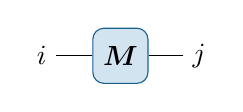
\begin{tikzpicture}[x=2cm, y=2cm]

\node [site] (M) at (0, 0) {$\bm{M}$};
\node (i) at (-0.5, 0) {$i$};
\node (j) at ( 0.5, 0) {$j$};

\draw (M) -- (i);
\draw (M) -- (j);

\end{tikzpicture}
\end{document}
